\documentclass{myclass}

\begin{document}

\subsubsection*{Zadanie 1.} 
Dwa psy ciągną sanie. W chwili pokazanej na rysunku prędkości psów są skierowane
wzdłuż lin i mają wartości \(v_1\) i \(v_2\). Liny tworzą ze sobą kąt
\(\alpha\). Oblicz wartość prędkości \(V\) sanek.
\begin{figure}[h!]
    \centering
    \includegraphics[scale=0.2]{figs/Bez tytułu.png}
    \label{fig:my_label}
\end{figure}

\subsubsection*{Zadanie 2.} 
Prostopadłościenny, jednorodny blok skalny o masie \(M\) o podstawie kwadratu o
boku \(b\) i wysokości \(h>b\) spoczywa na ziemi. Krawędzie bloku są lekko
zaokrąglone. O krawędź bloku (na środku tej krawędzi) oparto lekką drabinę,
której drugi koniec spoczywa na ziemi w odległości \(b\) od bloku. Na drabinę
zaczął powoli wchodzić człowiek o masie \(m\) (wymiary człowieka można przyjąć
za bardzo niewielkie). W trakcie wspinaczki nie występowało tarcie między
drabiną a blokiem, lecz drabina się nie poruszała. Blok także był nieruchomy,
jednak w pewnym momencie w trakcie wspinaczki człowieka blok zaczął się
przewracać (obracać wokół jednej z krawędzi bez przesuwania po ziemi). Wyznacz
warunek, który muszą spełniać parametry \(M\), \(m\), \(b\) i \(h\) oraz
minimalny współczynnik tarcia \(\mu\) bloku o ziemię, dla którego opisana
sytuacja jest możliwa.

\subsubsection*{Zadanie 3.}
Jeden koniec jednorodnego pręta o długości \(l\) jest przyczepiony do sufitu w
punkcie \(A\) za pomocą lekkiej nici również o długości \(l\). Drugi koniec
pręta (\(B\)) spoczywa na gładkiej podłodze. W chwili początkowej odcinek \(AB\)
jest prostopadły do sufitu i \(|AB|=H\), przy czym zachodzi \(l<H<2l\).
Następnie koniec pręta zaczyna ślizgać się po podłodze w taki sposób, że nić
jest stale napięta. Wyznacz maksymalną szybkość środka masy pręta podczas
dalszego ruchu.
\begin{center}
    \includegraphics[scale=0.3]{figs/mech.png}
\end{center}

\subsubsection*{Zadanie 4.}
A light rod with length \(l\) is connected to the horizontal surface with a
hinge; a small sphere of mass \(m\) is connected to the end of the rod.
Initially the rod is vertical and the sphere rests against the block of mass
\(M\). The system is left to freely move and after a certain time the block
loses contact with the surface of the block — at the moment when the rod forms
an angle \(\phi=\pi/6\) with the horizontal. Find the ratio of masses \(M/m\)
and the velocity \(V\) of the block at the moment of separation.

\subsubsection*{Zadanie 5.} 
Gaz jednoatomowy jest ogrzewany w taki sposób, że jego ciepło molowe wynosi
\(2R\). Podczas ogrzewania objętość gazu podwoiła się. Jak zmieniła się
temperatura gazu?

\subsubsection*{Zadanie 6*.}
Wyznacz stosunek pojemności bardzo cienkiego, przewodzącego dysku o promieniu
\(R\) do pojemności przewodzącej kuli o takim samym promieniu.

\subsubsection*{Zadanie 7*.}
 Rozstrzygnij, czy pojemność powłoki metalowej w kształcie półsfery o promieniu
 \(R\) jest większa, mniejsza, czy równa połowie pojemności powłoki sferycznej o
 takim samym promieniu.

\begin{figure}[ht]
    \centering
    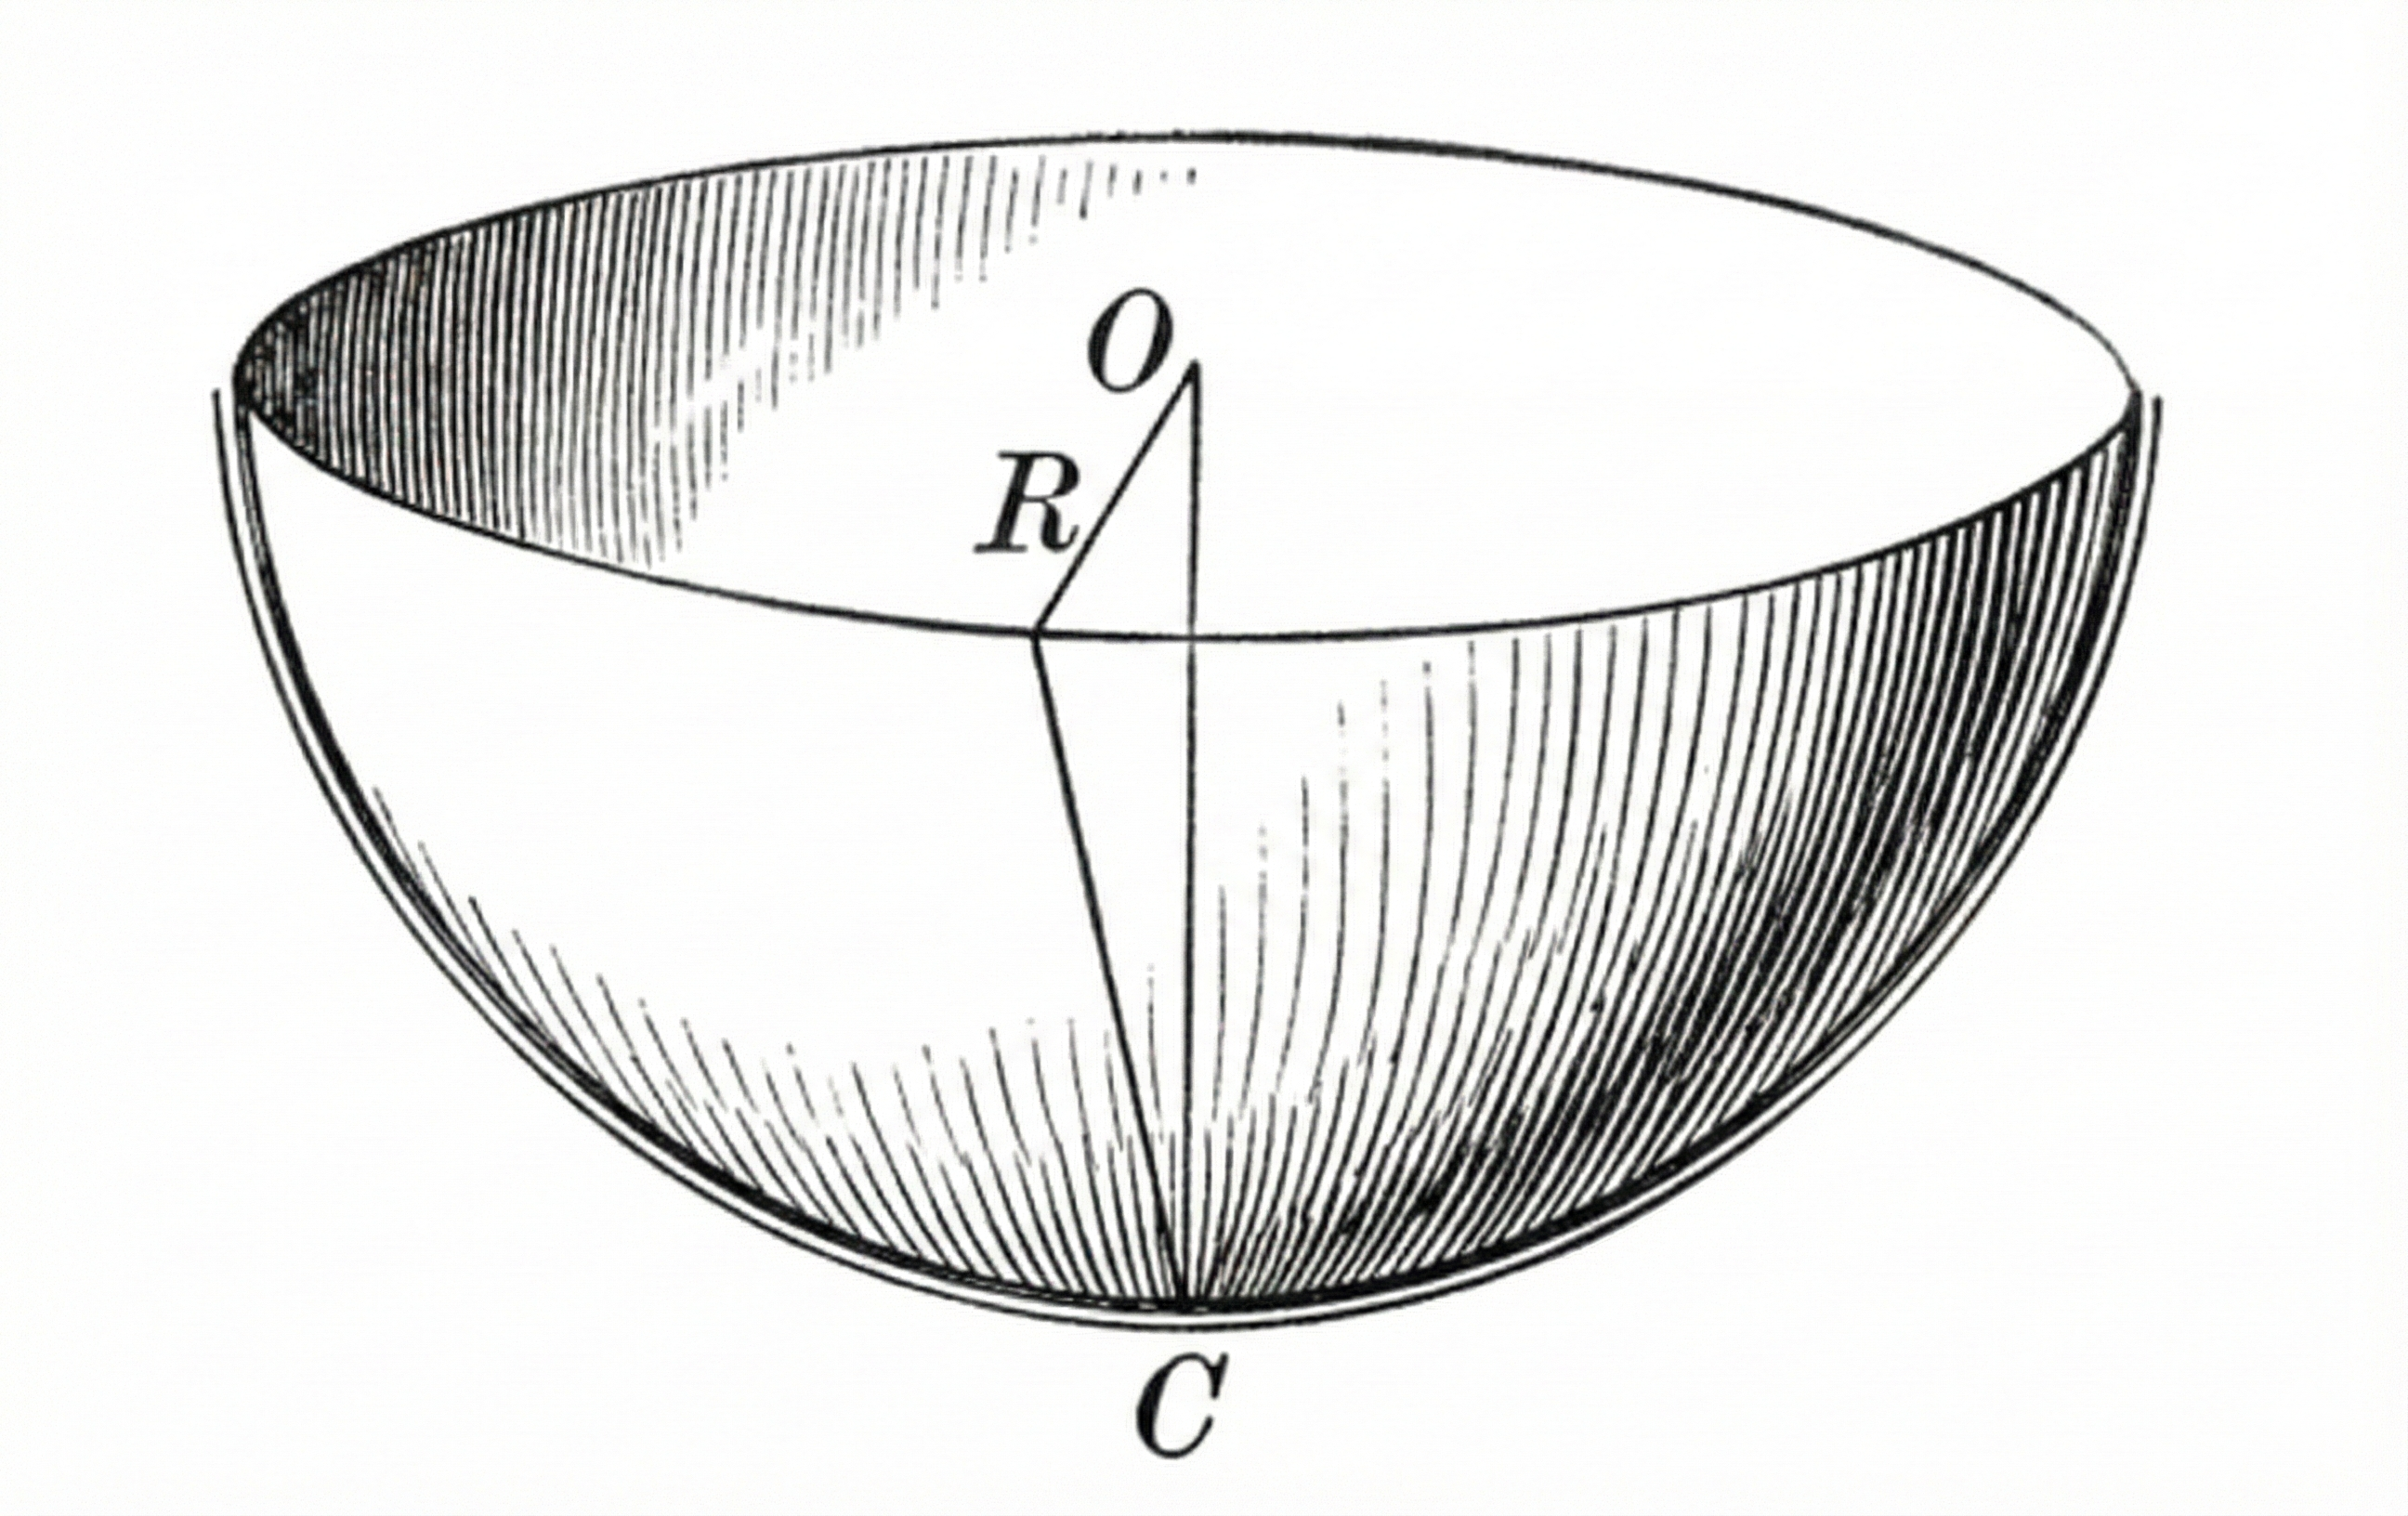
\includegraphics[scale=0.3]{figs/kelvin.png}
\end{figure}

\subsubsection*{Zadanie 8*.}
Jeden koniec sztywnego, nieważkiego pręta o długości \(l\) jest przymocowany do
punktu \((0,0,0)\), zaś do drugiego końca przymocowano niewielką kulkę o masie
\(m\) i ładunku \(q\). Cały układ znajduje się w nieważkości w jednorodnym polu
magnetycznym \(\mathbf{B}=[0,0,B]\) skierowanym pionowo do góry. Początkowo
kulka znajduje się w punkcie \((l,0,0)\) i ma prędkość \(\mathbf{v}_0=[0,0,v]\)
skierowaną pionowo do góry. Wyznacz maksymalną współrzędną \(z\) osiąganą przez
kulkę w trakcie jej ruchu.

\subsubsection*{Zadanie 9.}

Dwie równoległe, ustawiono pionowo metalowe, kwadratowe płyty o boku \(a\), są
utrzymywane nad powierzchnią nieprzewodzącej cieczy o gęstości \(\rho\), tak że
ich dolne krawędzie dotykają powierzchni cieczy. Płytki są w odległości \(d\) od
siebie. Po podłączeniu płytek do akumulatora, który utrzymuje stałe napięcie
\(U\), ciecz unosi się między płytami, ledwo sięgając ich górnych krawędzi.
Oblicz stałą dielektryczną cieczy. Pomiń wpływ napięcia powierzchniowego.

\subsubsection*{Zadanie 10.}

Pocisk wystrzelony z ziemi eksplodował na trzy fragmenty o równej masie w
najwyższym punkcie trajektorii. Jeden z fragmentów spadł po czasie \(\tau\)
(licząc od chwili wybuchu); pozostałe dwa fragmenty upadły jednocześnie po
czasie \(2\tau\) od chwili wybuchu. Oblicz wysokość, na jakiej eksplodował
pocisk.

\subsubsection*{Zadanie 11.}
Statek kosmiczny w kształcie stożka wykorzystuje ciśnienie promieniowania
słonecznego do oddalania się od Słońca. Oś stożka wskazuje bezpośrednio na
Słońce. Stożkowa powierzchnia statku jest pomalowana na czarno. Astronauci
próbują następnie zwiększyć swoje przyspieszenie, pokrywając powierzchnię
stożkową materiałem silnie odbijającym światło. Ku ich przerażeniu
przyspieszenie zmniejsza się o 30\%. Oblicz kąt rozwarcia stożka.

\subsubsection*{Zadanie 12.}
7 niewielkich identycznych kul (każda o masie \(m\)) o numerach 1,2,...,7
zostało połączonych w łańcuch (połączono pary (1,2), (2,3),..., (6,7)) lekkimi
pętami (o długości \(l\) każdy). Połączenia kul z prętami były ruchome (tj.
pręty połączone z jedną kulą mogły się obracać wokół kuli niezależnie od
siebie). Następnie unieruchomiono skrajne kule w odległości \(L\) od siebie (na
tej samej wysokości), pozwalając reszcie kul zwisać swobodnie. Okazało się, że
pręt łączący kule o numerach 3 i 4 był nachylony pod kątem \(30^\circ\) do
poziomu. Wyraź wartość \(L\) za pomocą \(l\).

\subsubsection*{Zadanie 13.}
Dany jest metalowy pręt, którego przekrój poprzeczny jest kołem o promieniu
\(r\). Pręt ten wygięto w obręcz o promieniu \(R\gg r\), przy czym końce pręta
były od siebie odległe o \(d\ll r\), zaś powierzchnie końców pręta były płaskie
i równoległe do siebie. Metal, z którego wykonano pręt, ma rezystywność
\(\varrho\), zaś obręcz ma masę \(m\). Obręcz tę umieszczono w obszarze, w
którym składowa \(z\) pola magnetycznego wynosi \(\alpha z\) dla pewnej stałej
\(\alpha\) i pole to wykazuje symetrię obrotową wokół osi \(z\). Obręcz była
prostopadła do osi \(z\), przy czym oś \(z\) byłą osią symetrii obręczy. W
chwili \(t=0\) przez obręcz nie płynął prąd, zaś współrzędna \(z\) jej środka
wynosiła \(z_0\). Przyspieszenie grawitacyjne było stałe, skierowane przeciwnie
do osi \(z\) i równe co do wartości \(g\). Obręcz spadała swobodnie, nie
obracała się, ani nie doformowała. Okazało się, że przyspieszenie obręczy
zależało od czasu zgodnie z następującym wzorem
\begin{equation*}
    a(t)=A+Be^{Ct}\,.
\end{equation*}
Wyznacz stałe \(A\), \(B\), \(C\).

\subsubsection*{Zadanie 14.}
Na rysunku wszystkie trzy woltomierze są idealne i jednakowe. Każdy opornik ma
taki sam opór \(R\). Napięcie na baterii wynosi \(U\). Oblicz wskazania
poszczególnych woltomierzy.
\begin{figure}[ht]
     \begin{center}
      \begin{circuitikz}[american voltages, scale=0.7]
      \draw
      (0,0) to [battery] (6,0) to [short] (6,2) to [generic,*-*] (4,2) to
      [generic,*-*] (2,2) to [generic, *-*] (0,2) to [short] (0,0) (2,4) to
      [voltmeter, l_=$V_2$] (2,2) (2,4) to [voltmeter, l=$V_3$,*-] (4,4) to
      [short] (4,2) (6,2) to [short] (6,6) to [generic] (4,6) to [generic] (2,6)
      to [generic, *-] (0,6) to [short] (0,4) (2,6) to [voltmeter, l_=$V_1$]
      (2,4) (0,4) to [short] (0,2);
      \end{circuitikz}
  \end{center}
     \label{fig:circuit1}
 \end{figure}

\subsubsection*{Zadanie 15.}
Wyznacz moment bezwładności jednorodnego prostopadłościanu o masie \(M\) i
krawędziach długości \(a\), \(b\), \(c\) względem osi obrotu zawierającej
najdłuższą przekątną prostopadłościanu.

\subsubsection*{Zadanie 16.}
Układ, którego schemat przedstawiono poniżej, zawiera idealne ogniwo i dwa
rezystory. Woltomierz użyty do pomiaru napięć na rezystorach i na baterii daje
następujące wskazania: 2 V, 3 V, 6 V. Jakie są rzeczywiste napięcia na
rezystorach w tym układzie?
\begin{figure}[ht]
     \begin{center}
      \begin{circuitikz}[american voltages, scale=0.8]
      \draw
      (0,0) to [battery] (6,0) to [short] (6,2) to [generic, l_=$R_2$] (3,2) to
      [generic, l_=$R_1$] (0,2) to [short] (0,0);
      \end{circuitikz}
  \end{center}
     \label{fig:circuit2}
 \end{figure}

\subsubsection*{Zadanie 17.}
Na poniższym rysunku każdy prostokąt oznacza rezystor o oporze \(1\,\Omega\).
Wyznacz opór zastępczy między punktami \(A\) i \(B\).

\begin{figure}[ht]
    \centering
    \includegraphics[scale=0.3]{figs/crct3.png}
    \label{fig:circuit3}
\end{figure}

\subsubsection*{Zadanie 18*.}

\begin{figure}[ht]
    \centering
    \includegraphics[scale=0.28]{figs/herring.png}
    \label{fig:Hering}
\end{figure}

Consider the system depicted in the picture below. The galvanometer remains
fixed in the lab, while the magnet is moved towards the galvanometer and the
tips of the leads slide around it. Determine total charge \(Q\) which passed
through the galvanometer if the areas of magnet and loop are \(A_1\), \(A_2\)
and the resistance of the galvanometer is \(R\).

\subsubsection*{Zadanie 19.}
Rozważmy dwie kule o promieniach \(a\), \(b\), które przecinają się pod kątem
prostym (tj. płaszczyzny styczne do sfer w dowolnym punkcie ich przecięcia są
prostopadłe). Wykonano metalowy odlew zewnętrznej powierzchni takiej bryły. W
punkcie \(X\) w odległości \(c\) od środka kuli o promieniu \(a\) i odległości
\(d\) od środka kuli o promieniu \(b\) umieszczono ładunek punktowy o wartości
\(q\). Wyznacz całkowity ładunek wyindukowany na przewodniku, jeżeli metalowy
odlew został uziemiony.

\subsubsection*{Zadanie 20.}
Dana jest przezroczysta kula o promieniu \(R\). Współczynnik załamania światła
zależy od odległości \(r\) od środka kuli według wzoru
\begin{equation*}
    n(r)=\frac{R+a}{r+a}\,,
\end{equation*}
gdzie \(a>0\) jest stałą. Na kulę pod kątem \(\alpha\) pada promień światła.
Wyznacz najmniejszą odległość tego promienia od środka kuli.

\subsubsection*{Zadanie 21*.}
Dana jest cienka powłoka sferyczna o promieniu \(R\). Gęstość powierzchniowa
masy powłoki w dowolnym punkcie \(P\) jest dana zależnością
\begin{equation*}
    \sigma(P)=\frac{\lambda}{SP^3}\,,
\end{equation*}
gdzie \(\lambda\) jest stałą, a \(S\) jest pewnym ustalonym punktem wewnątrz
powłoki sferycznej (możesz uznać, że znane są jego współrzędne). Wiedząc, że
odległość między punktem \(S\) i środkiem powłoki \(C\) wynosi \(f\) wyznacz
siłę działającą na jednostkową masę punktową umieszczoną w punkcie \(X\) na
zewnątrz powłoki, takim, że \(SX=CX=d\).

\subsubsection*{Zadanie 22*.}
In 1939, Cullwick reported an experiment, sketched above/below, in which a
steady current \(I\) flowed in a fixed wire along the axis of an annular metal
cylinder that moved with velocity \(v\) parallel to its axis. A galvanometer was
connected to contacts on the inner and outer radii of the cylinder, which
contacts remain fixed in the lab as the cylinder slid past them. Cullwick found
that reading of the galvanometer \underline{did not} depend on the permeability
of the cylinder, which could be made of copper or of iron. Explain theoretically
the results of the described experiment and calculate the measured EMF assuming
that the cylinder had inner radius \(a\) and outer radius \(b\).
\noindent\rule[0.5ex]{\linewidth}{1pt} Rozważmy eksperyment, którego schemat
został przedstawiony na poniższym rysunku. Przez bardzo długi prostoliniowy
przewód płynie stały prąd o natężeniu \(I\). Przewód ten znajduje się na osi
krótkiej, cylindrycznej rury o promieniu wewnętrznym \(r_1\) i zewnętrznym --
\(r_2\), która porusza się z szybkością \(v\) równolegle do swojej osi.
Galwanometr o rezystancji \(R\) jest podłączony do szczotek na wewnętrznej i
zewnętrznej powierzchni rury, przy czym szczotki pozostają w spoczynku w
laboratoryjnym układzie odniesienia, a odcinek je łączący jest prostopadły do
osi rury. W pierwszym eksperymencie wykorzystano rurę wykonaną z miedzi o
względnej przenikalności magnetycznej \(\mu_1\), natomiast w drugim
eksperymencie wykorzystano rurę wykonaną z żelaza o względnej przenikalności
magnetycznej \(\mu_2>\mu_1\). Wyznacz ładunek, jaki przepłynął przez galwanometr
odpowiednio w pierwszym i drugim eksperymencie w czasie \(\tau\). W którym
eksperymencie zmierzono większy ładunek?

\begin{figure}[ht]
    \centering
    \includegraphics[scale=0.3]{figs/cullwick.png}
    \label{fig:cullwick}
\end{figure}

\subsubsection*{Zadanie 23*.}
W dwóch czarnych skrzynkach z zaznaczonymi wyprowadzeniami znajdują się
narysowane obwody elektryczne. Podaj warunki jakie muszą spełniać parametry
\(R_1\), \(R_2\), \(R_3\), \(R_4\), \(C\), \(C'\), aby niemożliwe było
rozróżnienie obu układów za pomocą jakichkolwiek zewnętrznych pomiarów
elektrycznych, tzn. dla dowolnego, zmiennego w czasie napięcia, przyłożonego do
końcówek, natężenie prądu będzie w obu przypadkach jednakowe.

\begin{figure}[ht]
    \centering
    \begin{circuitikz}[american voltages, scale=0.8]
    \draw (0,0) to [generic, l_=$R_1$, -*] (0,-2) to [short] (1,-2) to [generic,
    l=$R_2$] (1,-4) to [short, -*] (0,-4); \draw (0,-2) to [short] (-1,-2) to
    [C, l_=$C$] (-1,-4) to [short] (0,-4) to [short] (0,-5) {}; \draw (0,0) to
    [short, -o] (-1,0); \draw (0,-5) to [short,-o] (-1,-5);
    
    \draw (4,-1) to [short] (6,-1) to [generic,l=$R_4$] (6,-5); \draw (4,-1) to
    [short] (4,-1) to [generic, l_=$R_3$] (4,-3) to [C, l_=$C'$] (4,-5) to
    [short] (6,-5); \draw (4,-1) to [short,*-o] (3,-1); \draw (4,-5) to
    [short,*-o] (3,-5);
    
    \end{circuitikz}
    \label{fig:circuit4}
\end{figure}

\subsubsection*{Zadanie 24.}
Przewrócony ciężki stożkowy lejek postawiono na równej poziomej płaszczyźnie
pokrytej arkuszem gumy. Węższy otwór lejka zakończony jest cienką rurką, przez
którą można do wnętrza lejka nalewać wodę. Okazuje się, że woda zaczyna wyciekać
spod lejka, gdy wysokość jej poziomu w rurce (mierząc od podłoża) wynosi \(h\).
Oblicz masę lejka \(M\), jeśli pole przekroju jego szerszego otworu
spoczywającego na podłożu wynosi \(S\), a wysokość lejka (bez rurki) wynosi
\(H\).

\subsubsection*{Zadanie 25*.}
Udowodnij, że moment bezwładności jednorodnego sześcianu o masie \(M\) i
krawędzi długości \(a\) względem dowolnej osi przechodzącej przez środek masy
sześcianu wynosi \(\frac{1}{6}Ma^2\).

\subsubsection*{Zadanie 26*.}
Z materiału o rezystywności \(\varrho\) wykonano rezystor w kształcie stożka
ściętego o wysokości \(h\) i promieniach podstaw \(a\), \(b\) (\(a<b\)). Do
podstaw stożka przyłożono elektrody będące kołami o promieniach odpowiednio
\(a\) i \(b\). Wyznacz przybliżoną wartość rezystancji takiego układu. Podaj
warunki, jakie muszą spełniać parametry \(a\), \(b\), \(h\), aby wyznaczona
wartość była bliska wartości rzeczywistej.

\subsubsection*{Zadanie 27.}
Gładki, długi pręt tworzy kąt \(\alpha\) z podłożem. Niewielki pierścień o masie
\(m\) jest nanizany na pręt i może swobodnie się po nim ślizgać. Do pierścienia
przymocowana jest lekka nitka na końcu której znajduje się niewielka kulka o
masie \(M\). Początkowo pierścień jest unieruchomiony, a nić wisi pionowo.
Następnie pierścień zostaje puszczony. Wyznacz przyspieszenie kulki tuż po
zwolnieniu pierścienia.

\subsubsection*{Zadanie 28*.}
A long cylinder of radius \(R\) has uniform magnetization \(\mathbf{M}\)
transverse to its axis. Find the magnetic field \(\mathbf{B}\) inside the
cylinder.

\subsubsection*{Zadanie 29.}
Na płytkę szklaną grubości \(100,25\lambda\) pada prostopadle promień światła
laserowego, którego długość fali wewnątrz płytki wynosi \(\lambda\). Gdy światło
o natężeniu \(I\) pada na powierzchnię styku powietrze--szkło lub
szkło--powietrze, wiązka przechodząca będzie miała natężenie \(rI\) (dla pewnego
ustalonego \(0<r<1\)), zaś odbita \((1-r)I\). Wiązka odbita od granicy faz
szkło--powietrze od strony powietrza zmienia fazę o \(\pi\), zaś wiązka
przechodzące (w obie strony) lub odbite od granicy faz od strony szkła nie
zmieniają fazy. Wyznacz natężenie wiązki odbitej od płytki. Natężenie światła
jest proporcjonalne do kwadratu amplitudy natężenia pola elektrycznego w wiązce.
Przyjmij, że szkło nie pochłania światła.

\subsubsection*{Zadanie 30.}
W pojemniku wyposażonym w tłok znajduje się \(n\) moli dwuatomowego gazu
doskonałego o temperaturze \(T\). Pojemność cieplna pojemnika wynosi \(C\). Gaz
jest w doskonałym kontakcie termicznym z pojemnikiem -- wymienia z nim ciepło
bardzo szybko. Pojemnik jest izolowany termicznie od otoczenia (nie wymienia
energii cieplnej z otoczeniem w żaden sposób). Początkowo objętość gazu w
pojemniku wynosiła \(V\). Wyznacz pracę potrzebną do przesunięcia tłoka tak, by
objętość gazu zmniejszyła się do \(V/2\).

\subsubsection*{Zadanie 31.}
Ciężar \(p\) jest zawieszony na trzech stalowych drutach wykonanych z tego
samego materiału, przyczepionych do sufitu w punktach odpowiednio \(A\), \(B\),
\(C\). Punkt \(D\) jest miejscem połączenia wszystkich trzech drutów. Wyznacz
siły, jakimi rozciągane są poszczególne druty. Zaniedbaj masy drutów. Druty
spełniają prawo Hooke'a z bardzo dużym modułem Younga -- tzn. takim, że
wprawdzie rozciągnięcie każdego z drutów jest niezerowe, ale jest ono
zaniedbywalnie małe w porównaniu z odległością między dowolnymi dwoma danymi
punktami.

\subsubsection*{Zadanie 32.}
Sides of the heptagon are resistors of resistance \(1\,\Omega\) and the
diagonals are resistors of resistance \(2\,\Omega\). Find the full resistance
between two adjacent points as a rational number in \(\Omega\).

\subsubsection*{Zadanie 33.}
Na płaszczyźnie zaznaczono 25 punktów postaci \((x,y)\), gdzie
\(x,y\in\{1,2,...,5\}\). Każde dwa punkty odległe o \(1\) połączono rezystorem o
wartości \(1\,\Omega\) otrzymując kratę złożoną z 40 oporników. Wyznacz opór
zastępczy tego układu (jako wymierną liczbę wyrażoną w \(\Omega\)) między
punktami \((1,1)\) i \((5,5)\).

\subsubsection*{Zadanie 34*.}
W dużym jednorodnym ośrodku o współczynniku przewodzenia ciepła \(\kappa\)
znajduje się cienki dysk o promieniu \(a\) i bardzo dużej przewodności cieplnej.
W płaszczyźnie dysku umieszczono współśrodkową z nim, okrągłą pętlę o promieniu
\(a+\epsilon\), gdzie \(0<\epsilon\ll a\), wykonaną z drutu oporowego, którą
następnie podłączono do źródła napięcia. Moc cieplna wydzielana na elemencie
wynosiła \(P\). Wyznacz temperaturę dysku \(T_0\) w stanie stacjonarnym, tj.
stanie, w którym temperatura każdego punktu nie zależy od czasu. Przyjmij, że
temperatura w punkcie bardzo odległym od dysku wynosi \(T_\infty\). Pomiń
wymianę ciepła na skutek promieniowania.
\medskip

\noindent\textbf{Przewodzenie ciepła}\\
Niech \(T(\mathbf{r})\) będzie polem skalarnym opisującym rozkład temperatury w
przestrzeni w stanie ustalonym. Oznaczmy \(\mathbf{q}=-\nabla T\), wówczas jeśli
przez \(\Phi\) oznaczymy strumień \(\mathbf{q}\) przez pewną powierzchnię
zamkniętą to w jednorodnym ośrodku o przewodności cieplnej \(\kappa\) zachodzi
\begin{equation*}
    \Phi=\frac{P}{\kappa}\,,
\end{equation*}
gdzie \(P\) jest całkowitym ciepłem przepływającym przez tą powierzchnię
zamkniętą w jednostce czasu.
\medskip

\noindent\textbf{Wzory, które mogą być przydatne}
\begin{equation*}
    \int \frac{1}{\sqrt{1-x^2}}\dd{x}=\arcsin(x)+\text{const.}
\end{equation*}

\subsubsection*{Zadanie 35*.}
Consider a very wide sheet of sheet resistance \(\varrho\). Two small electrodes
are put on the sheet at points \(A\) and \(B\), a distance \(s:=|AB|\) apart.
The resistance between these electrodes is measured to be \(R_1\). The sheet is
then cut to become a circle of radius \(r\) centered at a point \(O\) so that
\(\arcangle AOB=\theta\) and \(|OA|=|OB|<r\). Denoting the new resitance between
the two electrodes by \(R_2\), find the resistance change \(\Delta
R:=|R_2-R_1|\).
\medskip

The resistivity of thin homogeneous isotropic electrically conducting sheet is
usually characterized by the \underline{sheet resistance}, here denoted as
\(\varrho\), which is the resistance between the opposing sides of a
square-shaped sheet.

\subsubsection*{Zadanie 36.}
Dana jest przezroczysta kula o promieniu \(R\) umieszczona w powietrzu, której
współczynnik załamania zmienia się radialnie. Światło wychodzące z punktu na
brzegu kuli biegnie wewnątrz niej po trajektorii opisanej we współrzędnych
biegunowych równaniem
\begin{equation*}
    r^2-2rb\sin\phi=R^2\,,
\end{equation*}
gdzie \(b\) jest pewnym parametrem. Wyznacz zależność współczynnika załamania
światła wewnątrz kuli \(n(r)\), dla którego opisana sytuacja jest możliwa,
zakładając, że \(n(R)=1\).

\subsubsection*{Zadanie 37.}
Jednorodna obręcz o masie \(m\) i promieniu \(R\) jest zawieszona na trzech
identycznych, nierozciągliwych, pionowych niciach o długości \(l>R\), w taki
sposób, iż płaszczyzna obręczy jest pozioma. Obręcz obrócono o niewielki kąt
wokół osi prostopadłej do płaszczyzny obręczy przechodzącej przez jej środek, a
następnie puszczono. Obręcz zaczęła wykonywać niewielkie drgania, przy czym
płaszczyzna obręczy była stale pozioma, choć poruszała się w osi pionowej.
Wyznacz częstość \(\omega\) tych drgań. W rozwiązaniu przyjmij \(1+\phi^2\approx
1\), gdzie \(\phi\) jest kątem obrotu obręczy wokół osi prostopadłej do jej
płaszczyzny przechodzącej przez jej środek.

\subsubsection*{Zadanie 38.}
Wyznacz moment bezwładności pełnego, jednorodnego dwunastościanu foremnego o
masie \(m\) i krawędzi długości \(a\), względem osi przechodzącej przez środki
geometryczne dwóch naprzeciwległych ścian. Wynik podaj w postaci \(f ma^2\),
gdzie \(f\) jest ułamkiem dziesiętnym zaokrąglonym do czterech cyfr po
przecinku.
\begin{center}
    \includegraphics[scale=2]{figs/stock-vector-pentagonal-dodecahedron-stereometric-composition.jpg}
\end{center}

\subsubsection*{Zadanie 39.}
Jednorodna rura w kształcie torusa o promieniu \(a\), powstałego przez obrót
okręgu o promieniu \(b\ll a\), zawiera dwa gazy doskonałe odseparowane dwoma
szczelnymi, cienkimi, walcowymi tłokami o promieniach \(b\), które mogą
przemieszczać się wzdłuż rury bez tarcia i nie przewodzą ciepła. Rura została
umieszczona w dużym zbiorniku zawierającym gorący płyn o stałej i jednorodnej
temperaturze. Zakładając, że przepływ ciepła przez materiał rury jest w każdej
chwili taki sam w każdym punkcie oraz że podgrzewanie rury jest powolne, wyznacz
temperaturę \(t_1\) pierwszego gazu w chwili, gdy temperatura drugiego gazu
wynosi \(t_2\). Początkowe temperatury gazów wynoszą odpowiednio \(T_1\),
\(T_2\), natomiast ich ciepła molowe przy stałej objętości wynoszą odpowiednio
\(C_1\), \(C_2\).

\subsubsection*{Zadanie 40.}
Spoczywający neutron (n) rozpada się na trzy nieoddziałujące ze sobą cząstki:
proton (p), elektron (e) i antyneutrino (\(\nu\)). Masy spoczynkowe
poszczególnych cząstek wynoszą odpowiednio \(m_\text{n}\), \(m_\text{p}\),
\(m_\text{e}\), \(m_\nu\) (konkretne wartości wyszukaj w dostępnych źródłach).
Niech \(\mathscr{E}_\text{e}\) będzie energią relatywistyczną elektronu
powstałego w opisanym rozpadzie. Wyznacz największą możliwą wartość
\(\mathscr{E}_\text{e}\) i odpowiadające jej szybkości antyneutrina i protonu.
\medskip

\subsubsection*{Zależności, które mogą być przydatne}
W mechanice relatywistycznej energia cząstki o masie spoczynkowej \(m\)
poruszającej się z prędkością \(\boldsymbol{\beta} c\) wynosi
\begin{equation*}
    \mathscr{E}=\frac{mc^2}{\sqrt{1-\beta^2}}\,.
\end{equation*}
W przypadku zderzeń i rozpadów całkowita energia relatywistyczna układu jest
zachowana i posiada ona własność addytywności tj. energia relatywistyczna układu
cząstek jest równa sumie energii relatywistycznych poszczególnych cząstek.
Analogiczne własności posiada pęd relatywistyczny zdefiniowany jako
\begin{equation*}
    \mathbf{p}=\frac{m\boldsymbol{\beta}c}{\sqrt{1-\beta^2}}
\end{equation*}
dla cząstki o masie spoczynkowej \(m\) poruszającej się z prędkością
\(\boldsymbol{\beta} c\).

\subsubsection*{Zadanie 41.}
Na bardzo długiej równi pochyłej o kącie nachylenia \(\alpha\) umieszczono
jednorodny walec o masie \(m\) i promieniu \(r\). Początkowo walec nie obraca
się, a jego prędkość wzdłuż równi wynosi \(v_0\) i jest skierowana w górę równi.
Współczynniki tarcia statycznego i kinetycznego między walcem i powierzchnią
równi wynoszą odpowiednio \(\mu_\text{s}\) i \(\mu_\text{k}\), przy czym
\(\mu_\text{s}>\mu_\text{k}\). Wyznacz największą wysokość \(h\) jaką osiągnie
walec względem początkowego położenia. Podaj wartość numeryczną dla
\(m=1\,\text{kg}\), \(r=10\,\text{cm}\), \(v_0=1\,\frac{\text{m}}{\text{s}}\),
\(\alpha=30^\circ\), \(\mu_\text{k}=0.2\).

\subsubsection*{Zadanie 42.}
Znaleźć i scharakteryzować wszystkie możliwe położenia równowagi jednorodnego
pręta o długości \(L\) i masie \(m\) umieszczonego między dwiema prostymi
tworzącymi z poziomem kąty odpowiednio \(\alpha\) i \(\beta\), przy czym
\(\alpha,\beta\in[0;\pi/2]\).
\begin{center}
    \includegraphics[scale=0.3]{figs/equilibrium.png}
\end{center}
\begin{center}
    \includegraphics[scale=0.3]{figs/ew.png}
\end{center}

\subsubsection*{Zadanie 43.}
Do cienkiej, jednorodnej obręczy o masie \(m\) i promieniu \(r\) przymocowano
bardzo małych rozmiarów ciężarek o masie także równej \(m\). Obręcz może
poruszać się w płaszczyźnie pionowej po poziomym stole w polu grawitacyjnym o
natężeniu \(g\). Jaki warunek musi spełniać współczynnik tarcia \(f\) między
stołem a obręczą, aby początkowo nieruchoma obręcz z ciężarkiem znajdującym się
w pozycji odpowiadającej \(\alpha=\pi/3\) rozpoczynała ruch bez poślizgu?
Zakładając spełnienie tego warunku oblicz przyspieszenie kątowe obręczy w chwili
początkowej.

\subsubsection*{Zadanie 44*.}
Udowodnij, iż potencjał grawitacyjny \(V\) w dowolnym punkcie na powierzchni
jednorodnej elipsoidy obrotowej o masie \(M\), powstałej na skutek obrotu elipsy
o półosiach długości \(a\), \(b\) (\(a\geq b\)) wokół jej półosi małej, spełnia
nierówność
\begin{equation*}
    -\frac{GM}{b}\leq V\leq-\frac{GM}{a}\,.
\end{equation*}
Zakładamy, że potencjał w nieskończoności wynosi 0.

\subsubsection*{Zadanie 45.}
Na części teoretycznej III--go etapu LII Olimpiady Fizycznej pojawiło się
następujące zadanie\footnote{Patrz:
\href{http://of.szc.pl/pdf/LII-IIIT1_rozw.pdf}{http://of.szc.pl/pdf/LII-IIIT1\_rozw.pdf}}:
\begin{displayquote}
Dwie półkule o promieniach \(R\), wykonane z izolatora, naładowano równomiernie
ładunkami o gęstościach objętościowych \(\rho_1\) i \(\rho_2\) i zbliżono do
siebie na bardzo niewielką odległość -- rysunek. Oblicz siłę wzajemnego
oddziaływania tych półkul.
\end{displayquote}
Udowodnij użyty w rozwiązaniu wzorcowym lemat, iż siłę oddziaływania tych półkul
można zapisać jako \(\mathbf{F}=\rho_1\rho_2\mathbf{f}\), gdzie \(\mathbf{f}\)
jest siłą oddziaływania półkul o równych i jednostkowych gęstościach
objętościowych ładunku.

\subsubsection*{Zadanie 46.}
Gdyby Ziemia nagle zatrzymała się w ruchu orbitalnym, to ile dni spadałaby na
Słońce? Potrzebne dane, jeżeli będą potrzebne, wyszukaj w dostępnych źródłach.

\subsubsection*{Zadanie 47.}
Na osi cienkiego, przewodzącego dysku o promieniu \(R\) umieszczono punktowy
ładunek elektryczny o wartości \(q\) w odległości \(h\) od jego środka. Wyznacz
różnicę \(\Delta Q\) między ładunkiem wyindukowanym na dysku po stronie
znajdującej się bliżej punktowego ładunku, a ładunkiem wyindukowanym po stronie
przeciwnej, jeżeli metalowy dysk został uziemiony.
\end{document}
